\documentclass{beamer}

\usepackage{appendixnumberbeamer}

\usetheme[numbering=fraction, progressbar=frametitle]{metropolis}
\usefonttheme{serif}

\makeatletter
\defbeamertemplate*{section page}{mytheme}[1][]{
  \centering
  \begin{minipage}{22em}
    \raggedright
    \begingroup
    \usebeamercolor[fg]{section title}
    \usebeamerfont{section title}
    \insertsectionhead\\[-1ex]
    \usebeamertemplate*{progress bar in section page}
    \par
    \endgroup
    \ifx\insertsubsectionhead\@empty\else%
      \begingroup
      \usebeamercolor[fg]{subsection title}%
      \usebeamerfont{subsection title}%
      \insertsubsectionhead
      \endgroup
    \fi
    \vskip0.5cm
    \ifstrempty{#1}{}{%
      \begingroup
      \footnotesize%
      #1%
      \endgroup
    }
  \end{minipage}
  \par
  \vspace{\baselineskip}
}
\makeatother

\newcommand{\sectiontext}[2]{
   \setbeamertemplate{section page}[mytheme][#2]
   \section{#1}
   \setbeamertemplate{section page}[mytheme]
}

\usepackage{algorithmicx}
\usepackage[noend]{algpseudocode}
\usepackage{minted}
\setminted{fontsize=\footnotesize}
\usemintedstyle{tango}

\usepackage{xpatch,letltxmacro}
\LetLtxMacro{\cminted}{\minted}
\let\endcminted\endminted
\xpretocmd{\cminted}{\RecustomVerbatimEnvironment{Verbatim}{BVerbatim}{}}{}{}

\usepackage{tikz}
\usetikzlibrary{positioning,decorations.pathreplacing,shapes}

\usepackage{booktabs}
\usepackage{siunitx}
\usepackage{stmaryrd}
\usepackage{amsmath}
\usepackage{amssymb}
\usepackage{csquotes}

\newcommand{\xnleftrightarrow}[1]{\stackrel{#1}{\nleftrightarrow}}

\title{Revealing Behaviours of Concurrent Functional Programs by Systematic Testing}
\date{March 2018}
\author{Michael Walker}

\newcommand{\dejafu}{D\'{e}j\`{a}~Fu}

\usepackage{fontspec}
\setmainfont{equity}[
  % Files
  Path      = \string~/s/fonts/equity/ ,
  Extension = .otf ,
  % Fonts
  UprightFont     = Equity Text A Regular ,
  UprightFeatures = { SmallCapsFont = Equity Caps A Regular } ,
  BoldFont        = Equity Text A Bold ,
  BoldFeatures    = { SmallCapsFont = Equity Caps A Bold } ,
  ItalicFont      = Equity Text A Italic ,
  BoldItalicFont  = Equity Text A Bold Italic ,
  % Features
  Numbers = OldStyle ]

\begin{document}
\maketitle

\begin{frame}{Introduction}
  I want to make it easier to write correct concurrent code.

  I'm going to talk about three contributions today:

  \begin{itemize}
  \item A tool for testing concurrent Haskell programs.
  \item A scheduling algorithm for (incomplete) randomised testing.
  \item A tool for discovering properties of stateful Haskell
    functions.
  \end{itemize}
\end{frame}

\sectiontext{\dejafu{}: Haskell Concurrency Testing}{Michael Walker and Colin Runciman.  \dejafu{}: A Concurrency Testing Library for Haskell.  In \emph{Proceedings of the 8th ACM SIGPLAN Symposium on Haskell}, Haskell 2015, pages 141--152.  ACM, 2015.}

\begin{frame}{The scope of the tool}
  \textbf{Out of scope:} things which introduce nondeterminism beyond
  scheduler nondeterminism (+ relaxed memory).

  \textbf{In scope:} pretty much everything else.
\end{frame}

\begin{frame}[fragile]{We use a typeclass abstraction for concurrency}
\begin{center}
\begin{cminted}{haskell}
class Monad m => MonadConc m where
  -- associated types:
  type MVar m :: * -> *

  -- and functions:
  newEmptyMVar :: m (MVar m a)
  putMVar  :: MVar m a -> a -> m ()
  readMVar :: MVar m a -> m a
  takeMVar :: MVar m a -> m a

  -- (more entries omitted)
\end{cminted}
\end{center}
\end{frame}

% use a better example here (relmem one?)
\begin{frame}[fragile]{Usage is very close to normal concurrent Haskell!}
\begin{center}
\begin{cminted}{haskell}
-- import our library instead of the
-- usual "Control.Concurrent"
import Control.Concurrent.Classy

-- program against "MonadConc" instead
-- of the usual "IO"
myFunction :: MonadConc m => m String
myFunction = do
  var <- newEmptyMVar
  fork (putMVar var "hello")
  fork (putMVar var "world")
  readMVar var
\end{cminted}
\end{center}
\end{frame}

\begin{frame}[fragile]{\ldots except that \dejafu{} can tell us things about it}
\begin{center}
\begin{cminted}{text}
> autocheck myFunction
[pass] Never Deadlocks
[pass] No Exceptions
[fail] Consistent Result
    "hello" S0----S1--S0--

    "world" S0----S2--S0--
\end{cminted}
\end{center}
\end{frame}

\begin{frame}{Under the hood is a standard model checking process}
\begin{center}
\begin{minipage}{.6\linewidth}
\begin{algorithmic}
\Function{Explore}{$\mathcal M,\ \mathcal P$}
  \State $s$ \hspace{0.22cm} := $s_{0}$
  \State $out$ := $[]$
  \Loop
    \State $(r, t)$ := \Call{Run}{$\mathcal M,\ \mathcal P,\ s$}
    \State $out$ \hspace{0.16cm} := $out$ ++ $[(r,t)]$
    \State \textbf{case} \Call{Step}{$s,\ t$} \textbf{of}
        \State\hspace{\algorithmicindent} \textbf{Just} $s'$ \hspace{0.25cm} $\rightarrow$ $s$ := $s'$
        \State\hspace{\algorithmicindent} \textbf{Nothing}   $\rightarrow$ \Return $out$
  \EndLoop
\EndFunction
\end{algorithmic}
\end{minipage}
\end{center}

Where $s_{0}$ is a distinguished initial state, \textsc{Run} executes
the program once, and \textsc{Step} produces a new state.
\end{frame}

\begin{frame}{Our semantic model for concurrency tracks four things}
  \begin{center}
    $\langle\texttt{C},~\texttt{B},~\texttt{H},~\texttt{T}\rangle
    \rightarrow
    \langle\texttt{C},~\texttt{B},~\texttt{H},~\texttt{T}\rangle$
  \end{center}

  \begin{itemize}
  \item \texttt{C}, the number of capabilities.
  \item \texttt{B}, the relaxed-memory buffer state.
  \item \texttt{H}, the heap.
  \item \texttt{T}, a collection of threads.
  \end{itemize}

  \textbf{Covers:} forking, yielding/delaying, unsynchronised shared
  state, memory barriers, synchronised shared state, mutexes, software
  transactional memory, and exceptions.
\end{frame}

\begin{frame}{We provide three different ways to explore schedules}
\begin{center}
\begin{tabular}{l|ll}
                          & \textbf{Complete} & \textbf{Incomplete} \\ \hline
\textbf{Deterministic}    & DPOR              & Bounded DPOR        \\
\textbf{Nondeterministic} &                   & Weighted Random     \\
\end{tabular}
\end{center}

Bounded DPOR is complete within its bounds, but will miss results
beyond the boundary.
\end{frame}

\begin{frame}{When does the order between two concurrency actions matter?}
  If there is any state where the order in which two actions are
  performed matters, the actions are dependent:

  \begin{center}
    $\langle\texttt{thread\_id},~\texttt{haskell}\rangle
    \nleftrightarrow
    \langle\texttt{thread\_id},~\texttt{haskell}\rangle$

    $\left(\exists S.\ \llbracket xy \rrbracket_{S} \neq \llbracket yx \rrbracket_{S}\right)
    \implies x \nleftrightarrow y$
  \end{center}

  In practice, we usually define a syntactic approximation which is
  cheaper to compute than by examining all possible states.
\end{frame}

\begin{frame}{We use a conditional dependency relation}
  \begin{center}
    $\langle\texttt{thread\_id},~\texttt{haskell}\rangle
    \xnleftrightarrow{\mathcal C}
    \langle\texttt{thread\_id},~\texttt{haskell}\rangle$

    $\left(\exists S \in \mathcal C.\ \llbracket xy \rrbracket_{S} \neq \llbracket yx \rrbracket_{S}\right)
    \implies x \xnleftrightarrow{\mathcal C} y$

    $\left(\exists \mathcal C.\ x \xnleftrightarrow{\mathcal C} y \right)
    \implies x \nleftrightarrow y$
  \end{center}

  Our dependency relation is \textbf{conditional}.

  For example, two \texttt{putMVar v} calls are independent if
  \texttt{v} is full: they'll both just block.
\end{frame}

\begin{frame}[fragile]{A Concern: Daemon Threads \hfill \footnotesize (1/2)}
\begin{center}
\begin{cminted}{haskell}
main = do
  v <- newEmptyMVar
  fork $ do
    myThreadId
    myThreadId
    putMVar v "hello"
  tryReadMVar v
\end{cminted}
\end{center}
%$

What happens if the scheduler prefers the execution of the main
thread?
\end{frame}

\begin{frame}{A Concern: Daemon Threads \hfill \footnotesize (2/2)}
\begin{columns}[t]
\begin{column}{0.25\textwidth}
\texttt{newEmptyMVar}\\
\texttt{fork}\\
\texttt{tryReadMVar}
\end{column}
\begin{column}{0.25\textwidth}
\texttt{newEmptyMVar}\\
\texttt{fork}\\
\texttt{myThreadId}\\
\texttt{tryReadMVar}
\end{column}
\begin{column}{0.25\textwidth}
\texttt{newEmptyMVar}\\
\texttt{fork}\\
\texttt{myThreadId}\\
\texttt{myThreadId}\\
\texttt{tryReadMVar}
\end{column}
\begin{column}{0.25\textwidth}
\texttt{newEmptyMVar}\\
\texttt{fork}\\
\texttt{myThreadId}\\
\texttt{myThreadId}\\
\texttt{putMVar}\\
\texttt{tryReadMVar}
\end{column}
\end{columns}

\noindent\makebox[\linewidth]{\rule{\paperwidth}{0.4pt}}

\begin{columns}[t]
\begin{column}{0.25\textwidth}
\texttt{Nothing}
\end{column}
\begin{column}{0.25\textwidth}
\texttt{Nothing}
\end{column}
\begin{column}{0.25\textwidth}
\texttt{Nothing}
\end{column}
\begin{column}{0.25\textwidth}
\texttt{Just "hello"}
\end{column}
\end{columns}

\vspace{0.5cm}
Redundancy!  Oh no!
\end{frame}

\begin{frame}{How do we know it's right?}
  The DPOR algorithm and relaxed memory model we use come from the
  literature, we just translated them into Haskell.

  We haven't attempted a proof of correctness of our implementation,
  our semantics, or our dependency relation.

  But we \textbf{do} check internal data invariants and have extensive
  tests.
\end{frame}

\begin{frame}{We have three case studies}
  \begin{itemize}
  \item We reproduce a known deadlock in the auto-update library.
  \item We identify and fix a deadlock in the monad-par library.
  \item We use property-based testing to reproduce a bug in the async
    library.
  \end{itemize}
\end{frame}

\begin{frame}{How well does it work?}
  \begin{displayquote}
    \hspace{-0.7cm} {\Huge ``}
    I'd like to add that dejafu tests are by far the most reliable
    tests in our suite, in my experience --- I am yet to see a
    concurrency bug that they didn’t spot, while some other tests
    missed them!
    \vspace{1em}

    \noindent\normalfont\footnotesize
    Email correspondence with a Tweag I/O developer.
  \end{displayquote}
\end{frame}

\begin{frame}{\dejafu{} contributions}
  We contribute:

  \begin{itemize}
  \item A tool for testing concurrent Haskell with relaxed-memory
    effects, supporting both DPOR and random scheduling.

  \item An operational semantics of and dependency relation for
    Haskell concurrency.
  \end{itemize}
\end{frame}

\section{Scheduling Algorithms}

\begin{frame}{Why use incomplete approaches at all?}
  DPOR is all well and good, but sometimes complete testing is too
  slow, even with bounds.

  We want to be able to get \textbf{some} degree of confidence that
  such large programs are correct.
\end{frame}

\begin{frame}{The standard PCT algorithm}
  \begin{enumerate}
  \item Assign each thread a distinct priority from
    $\{d, \ldots, d+n\}$.
  \item Uniformly pick integers $c_1, \ldots, c_{d-1}$ from
    $\{1, \ldots, k\}$.
  \item Schedule threads strictly according to their priorities.

    After executing the $c_i$-th step $(1 \leq i < d)$, change the
    priority of the thread that executed the step to $i$.
  \end{enumerate}

  Where $n$ is the number of threads, $k$ is maximum execution length
  of the program, and $d$ is the \textbf{bug depth}.
\end{frame}

\begin{frame}{Our new weighted random scheduling algorithm}
  \begin{enumerate}
  \item Assign each thread a weight from
    $\{w_{min}, \ldots, w_{max}\}$.
  \item Uniformly pick integers $c_1, \ldots, c_{d-1}$ from
    $\{1, \ldots, k\}$.
  \item Schedule threads by weighted random selection.

    After executing the $c_i$-th step $(1 \leq i < d)$, change the
    weight of the thread that executed the step to a new uniformly
    chosen weight.
  \end{enumerate}

  Where $k$ is maximum execution length of the program, and $w_{min}$
  and $w_{max}$ define the range of weights.
\end{frame}

\begin{frame}{A source of inspiration: swarm testing}
  \begin{displayquote}
    \hspace{-0.7cm} {\Huge ``}
    [C]onsider testing an implementation of a stack ADT that provides
    two operations, push and pop. [\ldots] imagine the stack
    implementation has a capacity bug, and will crash whenever the
    stack is required to hold more than 32 items.

    \vspace{1em}

    \noindent\normalfont\footnotesize
    Alex Groce et al. ``Swarm Testing''. In: Proceedings of the 2012
    International Symposium on Software Testing and Analysis. ISSTA
    2012. ACM, 2012, pp. 78–88.
  \end{displayquote}

  \textbf{Idea}: do weighted random scheduling with weight re-use.
\end{frame}

\begin{frame}{Overlap of bugs found by the different approaches}
\begin{center}
\begin{minipage}{0.3\textwidth}
  \centering
  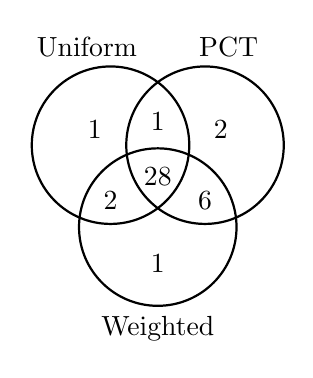
\begin{tikzpicture}[thick]
    \draw (0,0)      circle (1) node[above,shift={(-0.3,1)}] {Uniform};
    \draw (1.2,0)    circle (1) node[above,shift={(0.3,1)}]  {PCT};
    \draw (.6,-1.04) circle (1) node[below,shift={(0,-1)}]   {Weighted};

    \node at (.6,-.4)  {28}; % rand  ^ pct   ^ swarm
    \node at (1.2,-.7) {6};  % pct   ^ swarm - rand
    \node at (.6,.3)   {1};  % pct   ^ rand  - swarm
    \node at (0,-.7)   {2};  % rand  ^ swarm - pct
    \node at (1.4,.2)  {2};  % pct   - rand  - swam
    \node at (-.2,.2)  {1};  % rand  - pct   - swarm
    \node at (.6,-1.5) {1};  % swarm - pct   - rand
  \end{tikzpicture}

  \small Basic algorithms.
\end{minipage}
\hspace{2cm}
\begin{minipage}{0.3\textwidth}
  \centering
  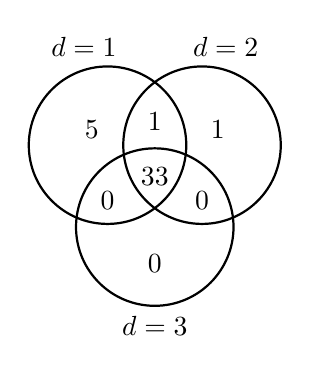
\begin{tikzpicture}[thick]
    \draw (0,0)      circle (1) node[above,shift={(-0.3,1)}] {$d=1$};
    \draw (1.2,0)    circle (1) node[above,shift={(0.3,1)}]  {$d=2$};
    \draw (.6,-1.04) circle (1) node[below,shift={(0,-1)}]   {$d=3$};

    \node at (.6,-.4)  {33}; % 1 ^ 2 ^ 3
    \node at (0,-.7)   {0};  % 1 ^ 3 - 2
    \node at (.6,.3)   {1};  % 1 ^ 2 - 3
    \node at (1.2,-.7) {0};  % 2 ^ 3 - 1
    \node at (-.2,.2)  {5};  % 1 - 2 - 3
    \node at (1.4,.2)  {1};  % 2 - 1 - 3
    \node at (.6,-1.5) {0};  % 3 - 1 - 2
  \end{tikzpicture}

  \small With weight changes.
\end{minipage}
\end{center}
\end{frame}

\begin{frame}{How rapidly bugs were found during execution}
\begin{center}
  \resizebox{0.9\textwidth}{!}{\input{gen/bugs-seminar.tex}}
\end{center}
\end{frame}

\begin{frame}{Swarm scheduling contributions}
  We contribute:

  \begin{itemize}
  \item Swarm scheduling, a scheduling algorithm for finding faults in
    concurrent programs.

  \item One parameterisation of swarm scheduling which performs as
    well as PCT, despite not knowing anything about the program under
    test.

  \item An argument, with evidence, that unfair schedules reveal
    concurrency bugs more effectively than fair schedules.
  \end{itemize}
\end{frame}

\sectiontext{CoCo: Discovering Concurrency Properties}{Michael Walker and Colin Runciman.  Cheap Remarks about Concurrent Programs.  Accepted for publication in: \emph{Functional and Logic Programming Symposium}, FLOPS 2018.  ACM, 2018.}

\begin{frame}{What sort of properties are we interested in?}
  Observational equivalence and strict observational refinement
  between Haskell terms operating on some distinguished shared state.

  \begin{center}
    \texttt{term1 ->- term2}

    \texttt{term1 === term2}
  \end{center}

  Where each term contains some state we know how to \textbf{observe}.
\end{frame}

\begin{frame}{We compare sets of program behaviours}
  For a term, we compute a mapping from \textbf{assignments to free
    variables} to a set of \textbf{pairs of observations and failure
    states}.

  \texttt{term1 === term2} if, for all assignments, the sets are
  equal.

  \texttt{term1 ->- term2} if there is at least one assignment where
  \texttt{term1} has a strict subset of the behaviours of
  \texttt{term2}, and for all other the sets are equal.
\end{frame}

\begin{frame}[fragile]{CoCo takes a user-supplied signature}
\begin{center}
\begin{cminted}{haskell}
sig = Sig
  { initialise  = maybe newEmptyMVar newMVar
  , expressions =
    [ lit "putMVar"  putMVar
    , lit "takeMVar" takeMVar
    , lit "readMVar" readMVar
    ]
  , backgroundExpressions =
    [ lit "tryPutMVar" tryPutMVar
    ]
  , interfere  = \v _ -> putMVar v 42
  , observe    = \v _ -> tryReadMVar v
  , backToSeed = \v _ -> tryReadMVar v
  }
\end{cminted}
\end{center}
\end{frame}

\begin{frame}[fragile]{Here are some MVar properties}
\begin{center}
\begin{cminted}{text}
   readMVar @  ->-  takeMVar @ >>= \x -> putMVar @ x
   readMVar @  ->-  takeMVar @ >>= \x -> tryPutMVar @ x
   readMVar @  ===  readMVar @ >> readMVar @
   readMVar @  ===  readMVar @ >> tryPutMVar @ x
   readMVar @  ===  readMVar @ >>= \x -> tryPutMVar @ x
   takeMVar @  ===  readMVar @ >> takeMVar @
  putMVar @ x  ===  putMVar @ x >> readMVar @
  putMVar @ x  ===  putMVar @ x >> tryPutMVar @ x1
\end{cminted}
\end{center}
\end{frame}

\begin{frame}[fragile]{Our expression representation}
\begin{center}
\begin{cminted}{haskell}
data Expr s h
  = Lit  String Dynamic
  | Var  TypeRep (Var h)
  | Bind TypeRep (Expr s h) (Expr s h)
  | Ap   TypeRep (Expr s h) (Expr s h)
  | State

data Var h = Hole h | Named String | Bound Int

type Schema s = Expr s ()
type Term   s = Expr s Void
\end{cminted}
\end{center}
\end{frame}

\begin{frame}[fragile]{One schema may have many term instances}
\begin{center}
\begin{cminted}{text}
f (? :: Int) (? :: Bool) (? :: Bool) (? :: Int)

f (w :: Int) (x :: Bool) (y :: Bool) (z :: Int)
f (w :: Int) (x :: Bool) (y :: Bool) (w :: Int)
f (w :: Int) (x :: Bool) (x :: Bool) (z :: Int)
f (w :: Int) (x :: Bool) (x :: Bool) (w :: Int)
\end{cminted}
\end{center}

We only need to evaluate the \textbf{most general term} to know the
results of all the others.
\end{frame}

\begin{frame}{The CoCo algorithm \hfill\footnotesize (1/2)}
\begin{center}
\begin{minipage}{\linewidth}
\begin{algorithmic}
\Function{Discover}{$\mathcal S,\ n$}
  \State $schemas$ := $[]$
  \For{$t \gets [1..n]$}
    \State $schemas[t]$ := \Call{Generate}{$\mathcal S,\ schemas,\ t$}
    \For{$s \gets schemas[t]$}
      \State $schemas[t][s]$ := \Call{Evaluate}{$s$}
      \For{$t' \gets [1..t]$}
        \For{$s' \gets schemas[t']$, where $schemas[t'][s'].smallest$}
          \State \Call{Properties}{$schemas[t][s],\ schemas[t'][s']$}
        \EndFor
      \EndFor
    \EndFor
  \EndFor
\EndFunction
\end{algorithmic}
\end{minipage}
\end{center}
\end{frame}

\begin{frame}{The CoCo algorithm \hfill\footnotesize (2/2)}
\begin{center}
\begin{minipage}{\linewidth}
\begin{algorithmic}
\Function{Properties}{$s,\ s'$}
  \State $properties$ := $[]$
  \For{$t \in s$}
    \For{$t' \in s'$}
      \For{$(r, r') \in$ \Call{Renamings}{$t, t'$}}
        \If{$r$ \texttt{->-} $r'$}
          \State $properties$ += $r$ \texttt{->-} $r'$
        \ElsIf{$r$ \texttt{===} $r'$}
          \State $properties$ += $r$ \texttt{===} $r'$
          \State $s.smallest$ := False
        \ElsIf{$r$ \texttt{-<-} $r'$}
          \State $properties$ += $r$ \texttt{-<-} $r'$
          \State $s.smallest$ := False
        \EndIf
      \EndFor
    \EndFor
  \EndFor
  \State \Call{Print}{$properties$}
\EndFunction
\end{algorithmic}
\end{minipage}
\end{center}
\end{frame}

\begin{frame}{Are the properties correct?}
  We only check a small number of free variable assignments, so CoCo
  has difficulty with wide types.

  We use \dejafu{} for determining term behaviours, so its correctness
  issues apply here too.

  \textbf{But,} the properties tend to be correct in practice.
\end{frame}

\begin{frame}{CoCo contributions}
  We contribute:

  \begin{itemize}
  \item A tool for discovering observational properties of stateful
    functions in the presence of concurrent interference.
\end{itemize}
\end{frame}

\begin{frame}[standout]
  Questions?
\end{frame}

\appendix

\sectiontext{Secret Prepared Answers Section}{Ha ha, you thought you had come up with a question I was unprepared for!}

\begin{frame}{\dejafu{}: Typeclass Overhead}
  \textbf{Is there an overhead of using typeclasses?}\\
  Yes.

  \textbf{Isn't that unfortunate for possibly performance-sensitive code?}\\
  Yes.

  \textbf{Do you have a solution?}\\
  Not really.  If I were starting \dejafu{} now I'd probably use backpack.
\end{frame}

\begin{frame}[fragile]{\dejafu{}: Testing Implementation}
\begin{center}
\begin{cminted}{haskell}
instance Monad n => MonadConc (ConcT r n) where
  type MVar (ConcT r n) = MVar r
  -- ...

  newEmptyMVarN n = toConc (ANewMVar n)

  putMVar  var a = toConc (\c -> APutMVar var a (c ()))
  readMVar var   = toConc (AReadMVar var)
  takeMVar var   = toConc (ATakeMVar var)
  -- ...
\end{cminted}
\end{center}
\end{frame}

\begin{frame}{\dejafu{}: Trace Rewriting}
  \textbf{Randomly generated traces are not nice:}\\
  \texttt{S0-----P1-P0----P2-P1-P0-P3-P1-S2-P3--P0-P3-P0-P3-}\\
  \texttt{S2-P0-S2-P0--P2-S0-}

  \textbf{But they can be simplified with some success:}\\
  \texttt{S0----------P1---S2--P3-----S0---S2---S0---}

  \textbf{We'd prefer this, though:}\\
  \texttt{S0------------S1---S0--S2-----S0--S3-----S0--}
\end{frame}

\begin{frame}[fragile]{\dejafu{}: Snapshotting}
\begin{center}
\begin{cminted}{haskell}
runForDCSnapshot :: (MonadConc n, MonadRef r n)
  => ConcT r n a
  -> n (Maybe (Either Failure (DCSnapshot r n a), Trace))

runWithDCSnapshot :: (MonadConc n, MonadRef r n)
  => Scheduler s
  -> MemType
  -> s
  -> DCSnapshot r n a
  -> n (Either Failure a, s, Trace)
\end{cminted}
\end{center}

One user reported a speed-up from 49.6s to 3.0s.
\end{frame}

\begin{frame}{\dejafu{}: The Heap}
  \textbf{Why use real mutable references in your implementation?}\\
  I agree that it's kind of nasty, as it means that my semantic
  function is not a pure function.

  But I tried using a heterogeneous map, and decided not to after
  seeing the overhead.  There's also a garbage collection problem: how
  do you know you can delete a key from your map?
\end{frame}

\begin{frame}{\dejafu{} / CoCo: Reasoning from Semantics}
  \textbf{Why run programs at all?  Why not just reason from the semantics?}\\
  I'm not modelling all of Haskell, only concurrency.

  The continuations \dejafu{} deals with are just regular Haskell
  functions.  I can't inspect them, all I can do is call them.
\end{frame}

\begin{frame}[fragile]{Swarm Scheduling: Algorithm}
\begin{center}
\begin{cminted}{c++}
void SwarmScheduler::Explore(State *init_state) {
  State *state = init_state;
  unsigned int steps = 0;

  while (!state->IsTerminal()) {
    AssignWeightsToNewThreads(state);

    auto it = PickNextRandom(state);
    for(unsigned int cpoint : changePoints) {
      if(steps == cpoint) {
        AssignWeightTo(it.first->uid());
      }
    }

    state = Execute(state, it.second);
    steps++;
  }
}
\end{cminted}
\end{center}
\end{frame}

\begin{frame}{CoCo: Interference}
  \textbf{What sort of interference is good?}\\
  Interference which does one, clear, thing (like \texttt{putMVar}),
  and running CoCo with many different types of interference.

  \textbf{Could you generate interference automatically?}\\
  Yes.  But I think it would be hard to do that in a way which doesn't
  violate assumed invariants.
\end{frame}

\begin{frame}[fragile]{CoCo: Evaluating Terms}
\begin{center}
\begin{cminted}{haskell}
runSCT' $ do
  let x = seedVal varassign
  s <- mkstate x
  r <- subconcurrency $ case interfere of
    Just interfereFunc -> do
      _ <- C.fork (interfereFunc s x)
      o <- eval_expr s
      pure o
    Nothing ->
      eval_expr s
  o  <- observe s x
  x' <- unstate s x
  pure (either Just (const Nothing) r, x', o)
\end{cminted}
\end{center}
\end{frame}

\begin{frame}{CoCo: Performance \hfill \footnotesize (1/2)}
\begin{center}
\begin{tabular}{lrrrrrrrr} \toprule
  Term size           &   3    &   4    &     5   &     6   &      7 &      8 \\ \midrule
  Schemas             &  56    &  88    &   238   &   385   &   1689 &   2740 \\
  Properties          &   0    &   0    &     1   &     1   &     55 &     55 \\
  Time (s)            &   0.45 &   0.45 &     9.2 &     9.2 &    970 &    970 \\ \midrule
  Time / schema$^{2}$ &  1.4e-4 & 5.8e-5 & 1.6e-4  & 6.2e-5  & 3.4e-4 & 1.3e-4 \\ \bottomrule
\end{tabular}
\end{center}
\end{frame}

\begin{frame}{CoCo: Performance \hfill \footnotesize (2/2)}
\begin{center}
    \begin{tabular}{lSSS} \toprule
      & {Time (s)} & {Max Residency (MB)} & {Properties} \\ \midrule
      \emph{All On}   &    945 & 250.6 & 55 \\
      \textbf{O1} Off &    965 & 250.6 & 55 \\
      \textbf{O2} Off &    994 & 261.7 & 59 \\
      \textbf{O3} Off &    983 & 254.3 & 55 \\
      \textbf{O4} Off &  99490 & 242.6 & 55 \\
      \emph{All Off}  & 102759 & 408.7 & 59 \\ \bottomrule
    \end{tabular}
\end{center}

  \raggedright \footnotesize
  \begin{description}
  \item[O1] is to exclude neutral schemas when generating larger schemas
  \item[O2] is to prune properties which are simple consequences of another
  \item[O3] is to only evaluate the most general term for each schema
  \item[O4] is to cache the behaviours of terms
  \end{description}
\end{frame}

\end{document}
